\chapter{XRemoteBot}\label{cha:xremotebot}

%fizxme NO EMPEZARIA CON ESTO... SINO CON UNA FUNDAMENTACION .. LA DESCRIPCION QUE HACES ACA LA PASARIA A LA SECCION DONDE EXPLICAS TU DESARROLLO

XRemoteBot es un servidor web que provee una API JSON para interactuar
con robots didácticos de forma remota y compartiendo un único enlace
físico con los robots. Está implementado en Python usando principalmente el
framework web Tornado, SQLAlchemy para acceder a la base de datos
y los módulos DuinoBot y Myro para
la comunicación con los robots. El cliente Javascript se encuentra
integrado con el servidor y la intensión es que sea utilizado desde una
vista web provista por el mismo, mientras que los clientes Python y Ruby
son independientes y la intensión es que sean utilizados en programas
tradicionales que se ejecuten desde fuera del navegador para enseñar
a programar en estos lenguajes usando un entorno habitual. XRemoteBot
es un rediseño y una reescritura completa de RemoteBot, un servidor
simple realizado como aplicación auxiliar de una aplicación Android
desarrollada
como trabajo práctico para la materia Laboratorio de Software.

\section{Remotebot}\label{sec:remotebot}

La versión original de Remotebot fue presentada como trabajo práctico
de la materia Laboratorio de
Software\footnote{\url{http://wiki.labmovil.linti.unlp.edu.ar/index.php?title=RemoteBot:_Android_\%2B_Robots}},
de esta Facultad,
el objetivo principal del trabajo era desarrollar una aplicación para
dispositivos Android que accediera a sensores y posiblemente a la red
wireless usando el lenguaje Java.

Para este trabajo se implementó
RemoteBot4Android\footnote{\url{https://github.com/fernandolopez/remotebot4Android}},
una aplicación Android
que permite controlar robots usando los acelerómetros de los dispositivos
móviles donde se ejecuta.

Una vez arrancado y configurado RemoteBot4Android se puede mover el robot
seleccionado inclinando el dispositivo en la dirección deseada o bien
detenerlo poniendo el dispositivo en posición horizontal. También es
posible controlar el robot sin utilizar los acelerómetros
con una botonera provista por la aplicación,
controlar la velocidad con un barra deslizante y ver la distancia al obstáculo
más cercano desde la interfaz.

El producto principal de este trabajo para la cátedra de Laboratorio de
Software fue el cliente
Remotebot4Android pero además del cliente, se desarrolló un
protocolo de comunicaciones
y un servidor básico que atiende los requerimientos y se los envía al
robot correspondiente, respondiendo también a peticiones de datos de
los sensores del
robot, ésta fue la primer implementación del servidor
Remotebot\footnote{\url{https://github.com/fernandolopez/remotebot}}
en cuyo concepto está basado XRemoteBot.

Remotebot provee una API JSON a través de HTTP que permite controlar a los
robots de forma remota, pero si bien es posible poner el servicio público,
el mismo no cuenta con autenticación, no soporta bien la concurrencia
y no provee ningún mecanismo de seguridad por lo que es recomendable solamente
usarlo dentro de ámbito de una red LAN.
La implementación del servidor
usa el módulo ``SimpleHTTPServer'' de la biblioteca estándar de Python para
proveer el soporte del protocolo HTTP e
introspección\footnote{\url{http://www.ibm.com/developerworks/library/l-pyint/}}.
para convertir los
mensajes enviados por los clientes en invocaciones a métodos.

\begin{figure}
    \centering
    \begin{subfigure}[b]{0.78\textwidth}
        \includegraphics[width=.95\textwidth]{figures/diagrama_remotebot}
        \subcaption{Diagrama de bloques de Remotebot}
        \label{fig:diagrama_remotebot}
    \end{subfigure}
    \begin{subfigure}[b]{0.2\textwidth}
        \centering
        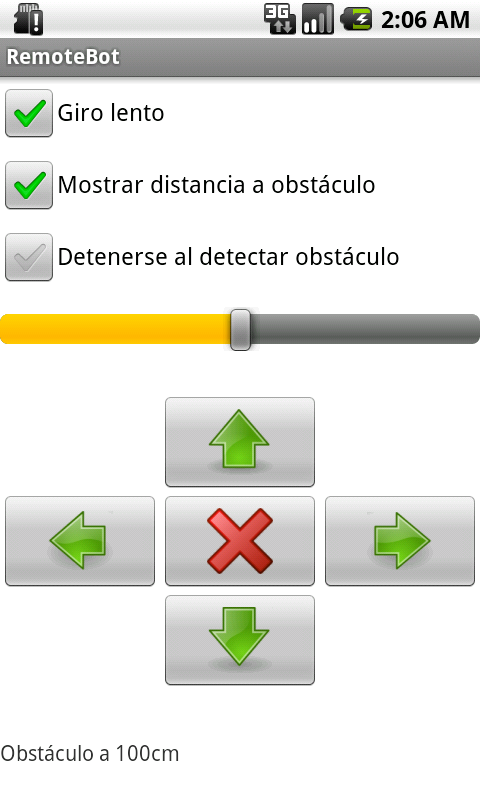
\includegraphics[width=\textwidth]{figures/cliente_remotebot}
        \subcaption{Cliente de Remotebot}
        \label{fig:cliente_remotebot}
    \end{subfigure}
    \caption{Diagrama de bloques e imagen del cliente Remotebot}
    \label{fig:diagrama_y_cliente_remotebot}
\end{figure}

Como se ve en la figura~\ref{fig:diagrama_remotebot} Remotebot utiliza la
biblioteca DuinoBot para comunicarse con los robots y el cliente para el cuál
fue diseñado es una aplicación Android que permite controlar los robots
y ver los valores del sensor de distancia usando una interfaz con botones,
además de poder controlar el robot usando los acelerómetros del dispositivo
(inclinar el dispositivo en una dirección dada hace que el robot se mueva
en esa dirección).

\section{XRemoteBot}\label{sec:xremotebot}

La interacción de XRemoteBot a nivel arquitectura es muy similar a la provista por Remotebot,
con la salvedad que el primero, además soporta robots Scribbler y puede ser
ampliado para interactuar con otros robots. Desde el punto de vista del cliente
XRemoteBot tiene varias diferencias, entre ellas la elección del protocolo,
usándose Websockets en lugar de peticiones HTTP y la definición del protocolo
de capa de aplicación que si bien es similar, ahora cuenta con un saludo y
un paso de autenticación a través de una ``API key''.

FIXME acá sé que falta más contenido del func. del servidor... (Fernando)

% FIXME donde estará el gráfico de esto?.
% me falta completar con la parte técnica de los módulos python
% usados, creo que algo de esto está escrito en otro capítulo
% lo tengo que pasar acá Fernando

\subsection{Modalidades del servidor}

A fin de hacer que el servidor pueda exponerse al público se cuenta con
un sistema con autenticación por \textit{API key}, pero estas claves
son largas resultando díficil recordarlas y escribirlas sin errores. En
ámbitos locales como puede ser una red wifi en un aula este mecanismo
de autenticación puede resultar molesto e innecesario, por lo que el
servidor es configurable de forma tal que se puede deshabilitar este
sistema de autenticación. Para que el servidor opere sin requerir
una \textit{API key} a los clientes basta con configurar la opción
\texttt{public\_server} en \texttt{False} dentro del archivo
\textit{configuration.py}.

% FIXME: Ampliar
% \chapter{WebSockets y Promises}\label{cha:websockets_y_promises}
% 
% Para el desarrollo de este trabajo decidió utilizar dos tecnologías
% que aún están en proceso de estandarización pero ya son ampliamente
% soportadas por distintos navegadores
% Web%
% ~\footnote{\url{http://caniuse.com/\#feat=websockets}}%
% ~\footnote{\url{http://caniuse.com/\#feat=promises}}
% como son la API
% \textit{WebSocket}~\footnote{La API en proceso de estandarización por la W3C,
% pero el protocolo ya fue estandarizado por IETF.}
% y la API \textit{Promise}~\footnote{En proceso de estandarización para
% ECMAScript 6 (Harmony).}.
% 
% En este capítulo se presenta una breve reseña de ambos y los motivos
% por los cuales fueron elegidos.

\subsection{WebSockets}\ref{sec:websockets}

Para permitir el uso remoto de los robots a través de Internet sin necesidad
de requerir configuraciones ni puertos especiales se eligió implementar el
sistema como una
aplicación web. Sin embargo, como se menciona en el
capítulo~\ref{cha:protocolo} no se utiliza HTTP para el intercambio de
mensajes y valores de retorno entre los clientes y el servidor sino el
protocolo WebSocket.

El protocolo WebSocket permite mantener conexiones persistentes y no envía
encabezados HTTP en cada mensaje, reduciendo así el overhead en los mensajes
intercambiados que supondría el uso de HTTP~\citep{wang_2013}, aprovechando al
mismo tiempo los puertos TCP que abre el servidor Web.

La elección de este protocolo trae como desventaja frente al uso de HTTP la
necesidad de tener consideraciones de seguridad especiales, para la parte
Web del sistema se utiliza autenticación con cookies pero no resulta seguro
utilizar el mismo mecanismo para la sesión con WebSockets ya que el sistema
quedaría vulnerable a ataques de tipo CSRF (Cross-Site Request
Forgery)~\citep{owasp_2014}~\footnote{
\url{https://www.owasp.org/images/5/52/OWASP_Testing_Guide_v4.pdf}}.

Una de las estrategias recomendadas es verificar el encabezado \texttt{Origin}
desde el servidor, pero esta técnica no es suficiente ya que los
clientes pueden falsear este campo y solamente si el cliente es un navegador
envía este encabezado.
Otra estrategia es tener un mecanismo de autenticación
separado para la comunicación~\footnote{\url{https://www.christian-schneider.net/CrossSiteWebSocketHijacking.html}},
esta fue la estrategia elegida para XRemoteBot usando una \textit{API key}
para identificar a los usuarios al inicio de la comunicación.

\section{Implementación de los clientes}

La implementación de XRemoteBot para esta tesina incluye tres clientes en distintos
lenguajes de programación: Python, Ruby y Javascript. Este último para ejecutarse
en el entorno de un navegador Web.

Estos clientes tienen distintas características y principalmente el que más difiere
de los otros es el cliente Javascript ya que es una implementación a ser ejecutada
en el navegador con las restricciones que esto trae, pero con la ventaja de que
se encuentra integrado con la vista Web de XRemoteBot por lo que cuenta con una
vista de la cámara al lado del campo de texto donde el usuario puede codificar.

En general se intentó copiar el estilo de programación del módulo DuinoBot original
de la forma más fiel posible, en el caso de Javascript por limitaciones del entorno
no se logró imitar este estilo tan fielmente como en los otros clientes.

\subsection{Cliente Python}\label{sec:python}
El uso del cliente Python es muy similar al uso directo de los robots con la
biblioteca DuinoBot aunque la implementación es bastante diferente por el protocolo
subyacente.

El cliente Python utiliza un solo módulo que no pertenece a la biblioteca estándar
de Python, el módulo para acceso a WebSockets
\textit{websocket-client}\footnote{\url{https://pypi.python.org/pypi/websocket-client}}
que cuenta, además de con una interfaz asincrónica, con una interfaz de ``bajo nivel''
sincrónica similar a la interfaz tradicional de Sockets.

\begin{lstlisting}[language=Python,
caption={Ejemplo con XRemoteBot para Python},label=lst:ejemplo_xremotebot_python]
from xremotebot import *
server = Server('ws://xremotebot.example:8000/api', 'api_key')
robot = Robot(server, server.fetch_robot())
robot.forward(100, 1)
robot.backward(50, 2)
print(robot.getObstacle())
\end{lstlisting}


Las operaciones con demoras, como los movimientos se implementan localmente
utilizando 2 mensajes y la función \texttt{time.wait()} de Python. De esta
forma
invocar al método \texttt{robot.forward(100, 1)} se traduce en los mensajes
de
la figura~\ref{fig:ejemplo_xremotebot_python_json}. Como todos los métodos
de movimiento
proveen esta funcionalidad de demora, la misma implementada en el
\textit{decorator}\footnote{Esto es un decorator de Python, no confundir
con el patrón de diseño. \url{https://www.python.org/dev/peps/pep-0318/}}
\texttt{xremotebot.timed} a fin de evitar repetición de código.

\begin{lstlisting}[language=Python,
caption={Mensajes generados al invocar \texttt{robot.forward(100, 1)} en
XRemoteBot para Python}, label=lst:ejemplo_xremotebot_python_json]
{
    "entity": "robot",
    "method": "forward",
    "args": [100]
}
# Después de 1 segundo...
{
    "entity": "robot",
    "method": "stop",
    "args": []
}
\end{lstlisting}


\subsection{Cliente Ruby}\label{ch4:ruby}

Las gemas que proveen soporte para WebSockets en Ruby proveen una API
asincrónica que no es deseable para este proyecto por lo que me incliné
por incorporar el código del
proyecto\footnote{\url{https://github.com/gimite/web-socket-ruby}}
al cliente Ruby de XRemoteBot, este proyecto no se encuentra empaquetado
en forma de gema pero provee una API sincrónica que permite implementar
el cliente Ruby de XRemoteBot para que se comporte de una forma muy similar
a la biblioteca DuinoBot original.

\begin{lstlisting}[language=Ruby,
caption={Ejemplo usando XRemoteBot para Ruby},
label=lst:ejemplo_xremotebot_ruby]
require 'xremotebot'
server = XRemoteBot::Server.new('xremotebot.example',
                                8000,
                                'api',
                                'api_key')

print "Robots #{server.get_robots}\n"
                                                                                                                    robot = Robot.new server, server.fetch_robot
robot.forward 100, 1
robot.backward 50, 2
print robot.getObstacle
\end{lstlisting}



\subsection{Cliente Javascript}\label{ch4:javascript}

\subsubsection{API Javascript y asincronismo}
Como se mencionó con anterioridad, gran parte de las decisiones de diseño de XRemoteBot
se hicieron para permitir la implementación de un cliente Javascript, pero dado el hecho
de que Javascript dentro del entorno de un navegador Web se comporta de forma asincrónica
no fue posible implementar un cliente Javascript cuyo uso se asemeje al de la biblioteca
de Python DuinoBot.

Para ilustrar esta problemática se puede tomar en consideración el 
código~\ref{lst:ejemplo_duinobot}
típico hecho usando DuinoBot en Python y analizar los inconvenientes para replicar
algo similar en Javascript.

\begin{lstlisting}[language=Python,
caption={Ejemplo típico usando DuinoBot},label=lst:ejemplo_duinobot]
from duinobot import *
board = Board()
robot = Robot(board, 10)
robot.forward(100, 1)
robot.backward(50, 2)
print(robot.getObstacle())
\end{lstlisting}


Las líneas 2 y 3 del ejemplo de la código~\ref{lst:ejemplo_duinobot} son
operaciones que retornan objetos, en XRemoteBot la línea 2 no tiene sentido
ya que la placa a la que está conectado el robot está predefinida en el
servidor, pero la línea 3 sí es necesaria para obtener una instancia de un
robot no reservado, estas operaciones que retornan un valor el XRemoteBot
se dividen en un mensaje de petición y uno de respuesta, el problema
es que por el asincronismo de Javascript y de la API de WebSockets no
es posible determinar en que momento llegará la respuesta con el valor
retornado y la única forma de bloquear la ejecución del script hasta que
llegue la respuesta sería hacer ``busy waiting'', lo cuál puede llegar a
bloquear la pestaña del navegador ya que los navegadores típicamente usan
un solo thread compartido entre el renderizado de la página, manejo de
eventos y ejecución del código Javascript asociado a la página.

En tanto las líneas 4 y 5 si bien no retornan un valor deben ejecutarse
en orden, y la línea 5 en este caso debe ejecutarse precisamente 1 segundo
después de la ejecución de la línea 4, también la línea 6 deberá ejecutarse
2 segundos después de la línea 5 ya que no es lo mismo preguntar si hay
un obstáculo cuando el robot aún no retrocedió, esto que parece muy obvio
y natural en la mayoría de los lenguajes de programación no es posible
en Javascript (dentro del navegador, con intérpretes como NodeJS sí es
posible) y el orden de ejecución y demora no se puede lograr simplemente
poniendo una instrucción debajo de otra.\footnote{FIXME}

\subsubsection{Promises}

Como se menciona en el la sección~\ref{sec:websockets} el servidor
utiliza Websockets como protocolo de transporte.
La API de WebSockets disponible en los navegadores Web requieren
redefinir una serie de funciones de la instancia del WebSocket
para recibir y enviar mensajes~\citep{websocket_2014}, a saber:
\begin{description}
    \item[\texttt{WebSocket\#onopen()}] se ejecutará cuando
    la conexión esté establecida.
    \item[\texttt{WebSocket\#onerror()}] se ejecutará ante un error en
    la conexión.
    \item[\texttt{WebSocket\#onclose()}] se ejecutará si la conexión
    se cierra.
    \item[\texttt{WebSocket\#onmessage()}] se ejecutará al recibir un
    mensaje desde el servidor, recibe como argumento el mensaje
    enviado por el servidor.
\end{description}

La intención del autor es ocultar estos detalles de implementación de
los usuarios que quieran controlar los robots usando la API Javascript,
para esto es posible utilizar el objeto \textit{Promise} que se encuentra
en proceso de estandarización para ECMAScript 6, pero ya se puede
usar en los navegadores más populares.

Los objetos \textit{Promise} se utilizan para obtener valores resultantes
de cómputos asincrónicos, como es el caso de la respuesta a una petición
hecha con WebSockets, la interfaz de \textit{Promise} no permite programar
los robots en Javascript con una interfaz idéntica a la usada al programar
los robots con la biblioteca DuinoBot, pero es relativamente fácil de
utilizar y ante la imposibilidad de demorar la ejecución del código
Javascript sin crear funciones adicionales provee una alternativa
relativamente simple en comparación con el uso directo de la interfaz
de los objetos \texttt{WebSocket}.

Los objetos \textit{Promise} se instancian pasándoles como argumento una
función que a su vez recibe 2 argumentos, \texttt{resolve} y \texttt{reject}.
El primer argumento ``cumple'' o ``resuelve'' la promesa y el segundo la
``rechaza''.
Las ``promesas'' tienen dos métodos: \texttt{then} y \texttt{catch} que se
ejecutan cuando la promesa se ``cumple'' o se ``rechaza'' respectivamente.

XRemoteBot para Javascript al crear cada mensaje le asigna un \texttt{msg\_id},
crea una \texttt{Promise} y guarda en un \texttt{object} de mensajes
pendientes un objeto que contiene las funciones \texttt{resolve} y
\texttt{reject} asociados con esa \texttt{Promise}
usando como clave el \texttt{msg\_id}. Al recibir una respuesta
desde el servidor, el cuerpo de \texttt{WebSocket\#onmessage()} toma el
\texttt{msg\_id} de la respuesta, lo utiliza para recuperar las funciones
asociadas con la \texttt{Promise} de este mensaje y ejecuta el
\texttt{resolve} pasándole como argumento la respuesta del servidor.
De esta manera las ``promesas'' asociadas con cada
mensaje se ``cumplen'' al obtener la respuesta correspondiente del servidor.

Cada método de XRemoteBot para Javascript que involucre enviar un mensaje
retornará una ``promesa'' que se cumplirá cuando el servidor responda
el mensaje.

Esto permite, por ejemplo, obtener el valor del sensor de distancia de un 
robot de forma simple como se ve en el código~\ref{lst:promises_get_obstacle}.
Si bien esta interfaz no es idéntica a la de DuinoBot, es lo más parecido
que se pudo lograr.

\begin{lstlisting}[language=C,
caption={Implementación de \texttt{getObstacle()} con ``promesas''},
label=lst:promises_get_obstacle]
robot.getObstacle().then(function(hay_obstaculo){
    if (hay_obstaculo.value){
        console.log("Hay un obstáculo al frente");
    }
    else {
        console.log("No hay obstáculos");
    }
});
\end{lstlisting}
% FIXME ta antes
La solución encontrada a este problema fue el uso de
\textit{Promises}~\citep{ECMA-262},
las \textit{Promises} proveen un mecanismo para ejecutar instrucciones,
que dependen de los resultados o de la terminación de eventos asincrónicos,
las \textit{Promises} permiten tener secuencia e interdependencia entre los
mensajes enviados a los
robots.
Si bien el objeto \textit{Promise} está en proceso de estandarización,
los navegadores Google Chrome, Firefox, Internet Explorer, Opera y Safari las
soportan\footnote{\url{https://developer.mozilla.org/en-US/docs/Web/JavaScript/Reference/Global_Objects/Promise}}.
El problema de esta solución es que la sintaxis de un script XRemoteBot en
Javascript usando \textit{Promises}
resulta bastante distinta de la sintaxis de un script DuinoBot como resulta
evidente
en el código~\ref{lst:ejemplo_xremotebot_javascript} donde se muestra un
script equivalente
al del código~\ref{lst:ejemplo_duinobot} escrito en Javascript.

\begin{lstlisting}[language=C,
caption={Ejemplo de XRemoteBot en Javascript},
label=lst:ejemplo_xremotebot_javascript]
var server = new Server('xremotebot.example:8000', 'api-key');
server.onConnect(function(){
    server.fetch_robot().then(function(robot){
        robot.forward(100, 1).then(function(){
            robot.backward(50, 2).then(function(){
                robot.getObstacle().then(function(obstacle){
                    println(obstacle);
                })
            })
        })
    });
});
\end{lstlisting}

Como se puede ver después de cada acción bloqueante, es decir cada método que
provoque una demora, y de cada método que retorne un valor útil, como
\texttt{Robot\#getObstacle()}, se invoca el método \texttt{Promise\#then()} con
una función anónima como argumento. Esta función que se pasa por argumento al
then se ejecutará si la \textit{Promise} se ``resuelve'', en el caso de
XRemoteBot la \textit{Promise} se ``resuelve'' cuando el servidor
responde al mensaje que generó la \textit{Promise}.
Este mecanismo se logró identificando cada mensaje con un \texttt{msg\_id},
manteniendo un objeto Javascript (usado como si fuera un \texttt{dict}
o \texttt{HashMap}) con el identificador como clave y la promesa
correspondiente a cada uno los mensajes cuyas respuestas están pendientes
como valor. Dentro del callback \texttt{onmessage} del WebSocket utilizado
al recibir una respuesta se busca el \texttt{msg\_id} en el objeto de
mensajes con respuesta pendiente y se ``resuelve'' la promesa correspondiente
a este mensaje. De esta manera se ejecuta la siguiente función (pasada como
argumento a \texttt{Promise\#then}) siguiendo con el flujo del programa
en orden y con la demora necesaria. En el
código~\ref{lst:ejemplo_xremotebot_javascript_promises} se muestra esta primer
implementación.


\begin{lstlisting}[language=C,
caption={Ejemplo simplificado de la implementación de XRemoteBot con
Promises dentro del constructor Server en remotebot.js},
label=lst:ejemplo_xremotebot_javascript_promises]
this.send_ws_msg = function(msg){
    var promise;
    promise = new Promise(function(resolve, reject){
        that.pending_msgs[msg_id] = {resolve: resolve, reject: reject};
    });
    msg['msg_id'] = msg_id;
    that.ws.send(JSON.stringify(msg));
    return promise;
}
// ...
this.ws.onmessage = function(msg){
    msg = JSON.parse(msg.data);
    if (msg['msg_id'] !== undefined){
        var executor = that.pending_msgs[msg['msg_id']];
        delete that.pending_msgs[msg['msg_id']];
        executor.resolve(msg);
    }
};
\end{lstlisting}


Evidentemente esta forma de programar resulta engorrosa y poco práctica,
por lo que se añadieron
lógica y estructuras de datos extra que serializan en envío de mensajes al
servidor, enviando de a un mensaje por vez (el objeto Javascript con
mensajes con respuesta pendiente tendrá a lo sumo una entrada)
y encolando los mensajes sobrantes
en una cola de mensajes demorados (\texttt{Server\#delayed}), cuando
el servidor contesta el mensaje enviado anteriormente se toma un mensaje
de la cola si lo hubiere y se lo envía al servidor. De esta manera
se garantiza la demora necesaria entre la ejecución de cada método
del robot, sin embargo para obtener los valores de retorno de los métodos,
como en el caso de los métodos de acceso a los sensores, sigue siendo
necesario el uso del método \texttt{Promise\#then}. A pesar de esto último
como se puede ver en el código~\ref{lst:ejemplo_xremotebot_javascript_cola}
con estas modificaciones es posible hacer que el cliente Javascript
tenga una API más limpia y usable, esta última versión es la definitiva
para este trabajo.

\begin{lstlisting}[language=C,
caption={Ejemplo de XRemoteBot en Javascript con empleo de una cola para
serializar mensajes},
label=lst:ejemplo_xremotebot_javascript_cola]
var server = new Server('xremotebot.example:8000', 'api-key');
server.fetch_robot().then(function(robot){
    robot.forward(100, 1);
    robot.backward(50, 2);
    robot.getObstacle().then(function(obstacle){
        println(obstacle);
    });
});
\end{lstlisting}


Una solución alternativa para lograr imitar tanto como sea posible la
API de DuinoBot puede ser utilizar un intérprete Javascript implementado en
Javascript como
JS-Interpreter\footnote{\url{https://github.com/NeilFraser/JS-Interpreter}},
pero requeriría modificar el intérprete para lograr una ejecución paso a paso
controlada por el flujo de mensajes a través de la conexión con WebSockets,
además de agregar complejidad, este tipo de intérpretes no accede a un entorno
compreto como lo hace el intérprete incorporado en los navegadores y puede
tener incompatibilidades o funcionalidades no implementadas, en este caso
por ejemplo JS-Interpreter no soporta interrupciones y no puede interactuar
directamente con DOM, otra opción es
Hypnotic\footnote{\url{http://coolwanglu.github.io/hypnotic/web/demo.html}}
que utiliza el intérprete Narcissus y provee una función \texttt{sleep()} que
demora la ejecución del código como se desea para este proyecto, pero el
invoveniente de Hypnotic es que por el momento solamente funciona en el
navegador
Firefox\footnote{\url{https://github.com/coolwanglu/hypnotic/wiki\#limitations}}.


\subsubsection{Interacción con DOM y JQuery}

Dado que este cliente se ejecuta en el entorno de un navegador Web es posible
interactuar con el árbol DOM de la página, por ejemplo modificando sus nodos y
dado que la interfaz Web utiliza JQuery esta biblioteca también está disponible
para los usuarios, pudiendo hacer por ejemplo un script que pide los valores
de los sensores de línea cada 500 milisegundos y los muestra en el título de la
página usando JQuery para manipular el árbol DOM como se ve en el
 código~\ref{lst:ejemplo_dom_title}.

\begin{lstlisting}[language=C,caption={Manipulación de DOM con JQuery desde
XRemoteBot para Javascript},label=lst:ejemplo_dom_title]
var server = new Server('ws://localhost:8000/api',
                        '97385401-3874-439c-b01b-df94349d888a');
server.onConnect(function(){
    server.fetch_robot().then(function(robot_obj){
        var robot = new Robot(server, robot_obj);
        setInterval(function(){
            robot.getLine().then(function(line){
                $('title').text('Sensor de línea: ' + line);
            });
        }, 500);
    });
});
\end{lstlisting}


\subsubsection{Interfaz Web y streaming de video}

La interfaz Web de XRemoteBot, que está pensada principalmente para los casos
de uso donde los clientes están en una ubicación geografica distinta a la de
los robots provee login, acceso a la visualización y renovación de una
clave alfanumérica única por cada usuario denominada \textit{API key} que
permite reservar y controlar los robots sin la necesidad de exponer el nombre
de usuario y contraseña, y una página que permite ver los robots en vivo por
video opcionalmente controlandolos con un script Javascript.


Esta interfaz provee un sistema para crear usuarios nuevos, obtener las
API key y acceso a la documentación básica para trabajar con XRemoteBot
desde cualquiera de los tres clientes implementados.

La interfaz web pensada principalmente para ser utilizada en conjunto
 con el cliente
Javascript, aunque puede ser accedida sin problemas aún si se usa
otro de los clientes para poder visualizar los robots a través del
streaming de video. Provee un area de texto para escribir los ejemplos
en Javascript, esta area de texto es creada con CodeMirror
que provee resaltado de sintáxis y manejo de los eventos de teclado para
que al presionar Tab el editor idente el código en lugar de saltar a otro
elemento de la página como harían los navegadores por defecto.

Otra area de texto en la parte inferior
 simula la salida de una terminal, en la misma
se pueden ver mensajes de log generados con la función
\texttt{rblog} que pueden ser habilitados o deshabilitados desde un
checkbox y mensajes impresos con la función \texttt{println}.

Un area de video destinada a emisiones en vivo que muestren la posición
del robot, el mismo no requiere ningún plugin ya que se utilizó
\texttt{jsmpeg}\footnote{\url{https://github.com/phoboslab/jsmpeg}}
que permite emitir video en vivo usando WebSockets y renderizarlo
en el navegador en un elemento Canvas, de esta manera se logró tener
video en vivo utilizando características estándar de HTML5.
